\chapter{Future work}

In this section we describe the stages that will be performed to achieve the objective declared in this thesis proposal as well as the description of the experimenters needed to validate (or disprove) the hypotheses of this work.:

\section{Data Bases Generation}
\label{sec_DB_Gen}

\emph{2-D} binary permeability channels will be used as target media. We will work under a stationary assumption for the channels. We will consider $3$ kinds of simplified channels (see fig. \ref{fig:Proposed_ChannelizedFields}): a single channel model and two multichannel models with different level of complexity. These models have the form of \emph{2-D} discrete images representing a realization of a real channel. The realizations of the models are obtained using the standard \emph{SGEMS} program (by \emph{SNESIM} algorithm) and an additional preliminary training image provided by an expert.
 	
Equipped with the \emph{SNESIM} algorithm we simulate realizations for each kind of channel. Each image have a size of $200$ by $200$ where each pixel with value $1$ represents a high permeability position. Selected images will be used as realizations images (\emph{RIs}) of the actual subsurface channels while others will play the role of training images (\emph{TIs}).
	
\section{Experimental Design}
\label{sec_Prop_Exp}

\subsection{Empirical Analysis of Classical Sampling Schemes and its Comparison with \emph{AdSEMES} }

We propose the analysis of both preferential and non-preferential sampling schemes. On the one hand, for non-preferential sampling methods, we consider classical rules such as: (1) uniform random sampling, (2) deterministic stratified sampling, (3) randomized stratified sampling, and (4) multiscale stratified sampling. On the second hand, for preferential sampling, (5) maximum indicator sampling, (6) oracle version of maximum entropy sampling, and (7) the proposed \emph{AdSEMES} rule are evaluated.

For the maximum indicator sampling, a coarse regular grid of samples is defined for the initial sampling stages. Then, iteratively, more detailed grid are sampled surrounding the locations at the coarser grid that achieves some predefined indicator (for example, presence of a channel or high permeability).

For the oracle version of maximum entropy sampling, the samples are taken close to the transition zones in the real image. This scheme aims to provide insights of the theoretical behavior of the proposed sampling rule. 

Given a sampling scheme, for each kind of field proposed in section \label{sec_DB_Gen}, an iterative sampling process of $400$ measurements (sampling rate from $0 \%$ to $1 \%$) will be performed. Then, using the appropriate training image defined in section \label{sec_DB_Gen} and the obtained measurements as conditioning hard data, $200$ realizations of the interest media will be simulated by \emph{MPS}.

In order to assess the performance of implemented methods, we will measure time required for the execution of each specific sampling strategy and we will study several metrics of overall performance from image reconstruction and entropy reduction. Particularly, for each sets of \emph{MPS} realizations, we propose to evaluate metrics such as: pixel mean, pixel variance, marginal entropy, and iso-probability maps in order to compare the performance of the sampling schemes under analysis.


\subsection{Simulation based Analysis to Study the Performance of \emph{OWP} under known Field Models}

To evaluate the goodness of \emph{OWP} under controlled conditions, we propose the study of several classical theoretical regionalized fields and propose an indicator of media complexity:
	\begin{itemize}
		\item {Resolvability Capacity (\emph{RC}): } We will define an indicator of media complexity based on the entropy reduction provided by the incorporation of \emph{OWP} positions to the measured knowledge of the field of interest.
		\item {Gaussian Fields and OWP: } We will study several common literature related with optimal sensor placement for continuous regionalized medias.
		\item {Markov Chains Modeling for Binary Maps: } We will study some models of spatial dependence based on Markov chains and to implement \emph{Cliqué} based principles in our \emph{OWP} framework.
		\item {\emph{RC} and Medias with Theoretic \emph{pdfs}: } We will study the behavior of \emph{RC} under some regionalized fields with classical theoretic \emph{pdfs}.
	\end{itemize}














	
	
	
\section{Implementation Aspects of the \emph{OWP} Algorithms} 
In order to conduct the experiments declared in section \ref{sec_Prop_Exp}, we will develop the next stages to implement the \emph{OWP} rule:

	\begin{itemize}
		\item {Entropy Estimation: }  Implementation of an empirical frequentist approach for entropy estimation from \emph{MPS} realizations.
		\item {Sequential \emph{OWP} Solver: } Implement the \emph{OWP} solver that find optimal spatial sensing positions using the principle presented in section \ref{sec_OWP_Form}.
		\item {Evidence based and sequential \emph{OWP}: } Implementation of a framework with re-simulation of \emph{MPS} using previous selected positions as hard data for conditioning the statistics as posted in section \ref{sec_Meth_Marginal}.
	\end{itemize}


\subsection{Extension of Proposed Algorithms} 

In the long term, we propose the following stages to improve the \emph{OWP} framework:
	\begin{itemize}
		\item {Patterns Analysis from TI:} We will modify our pattern analysis for \emph{pdfs} estimation bypassing \emph{MPS} by using the training images as a source of pattern occurrences on the channelized structure of interest. We will study several theories developed to address it problem.
		\item {TIPS Formulation:}  We will implement a training image based pattern search \emph{TIPS}.
		\item {OWP-TIPS Approach:} We will modify \emph{OWP} to incorporate \emph{TIPS} approach.
	\end{itemize}





















\section{Writing manuscripts for journals}

We propose to write two journal manuscripts and to assist some international conferences. The first will be focus on the presentation of the method, its algorithmic implementation and preliminary analysis of its performances under controlled conditions.

The second contribution will be focus on the application of this \emph{OWP} sampling scheme in the recovery of channelized fields and the way this approach improves the performance of \emph{MPS} algorithms.

%\newpage
\section{Gannt charts}


To organize preliminary and future work we provide two separate time tables. The first one oriented to our preliminary work related with this thesis proposal and the second one oriented to the current and future work for the next years. The preliminary work is summarized in fig. \ref{fig:RoadMap1}, and the future work can be seen in fig. \ref{fig:RoadMap2}.


\begin{figure}[ht!]
    \centering
    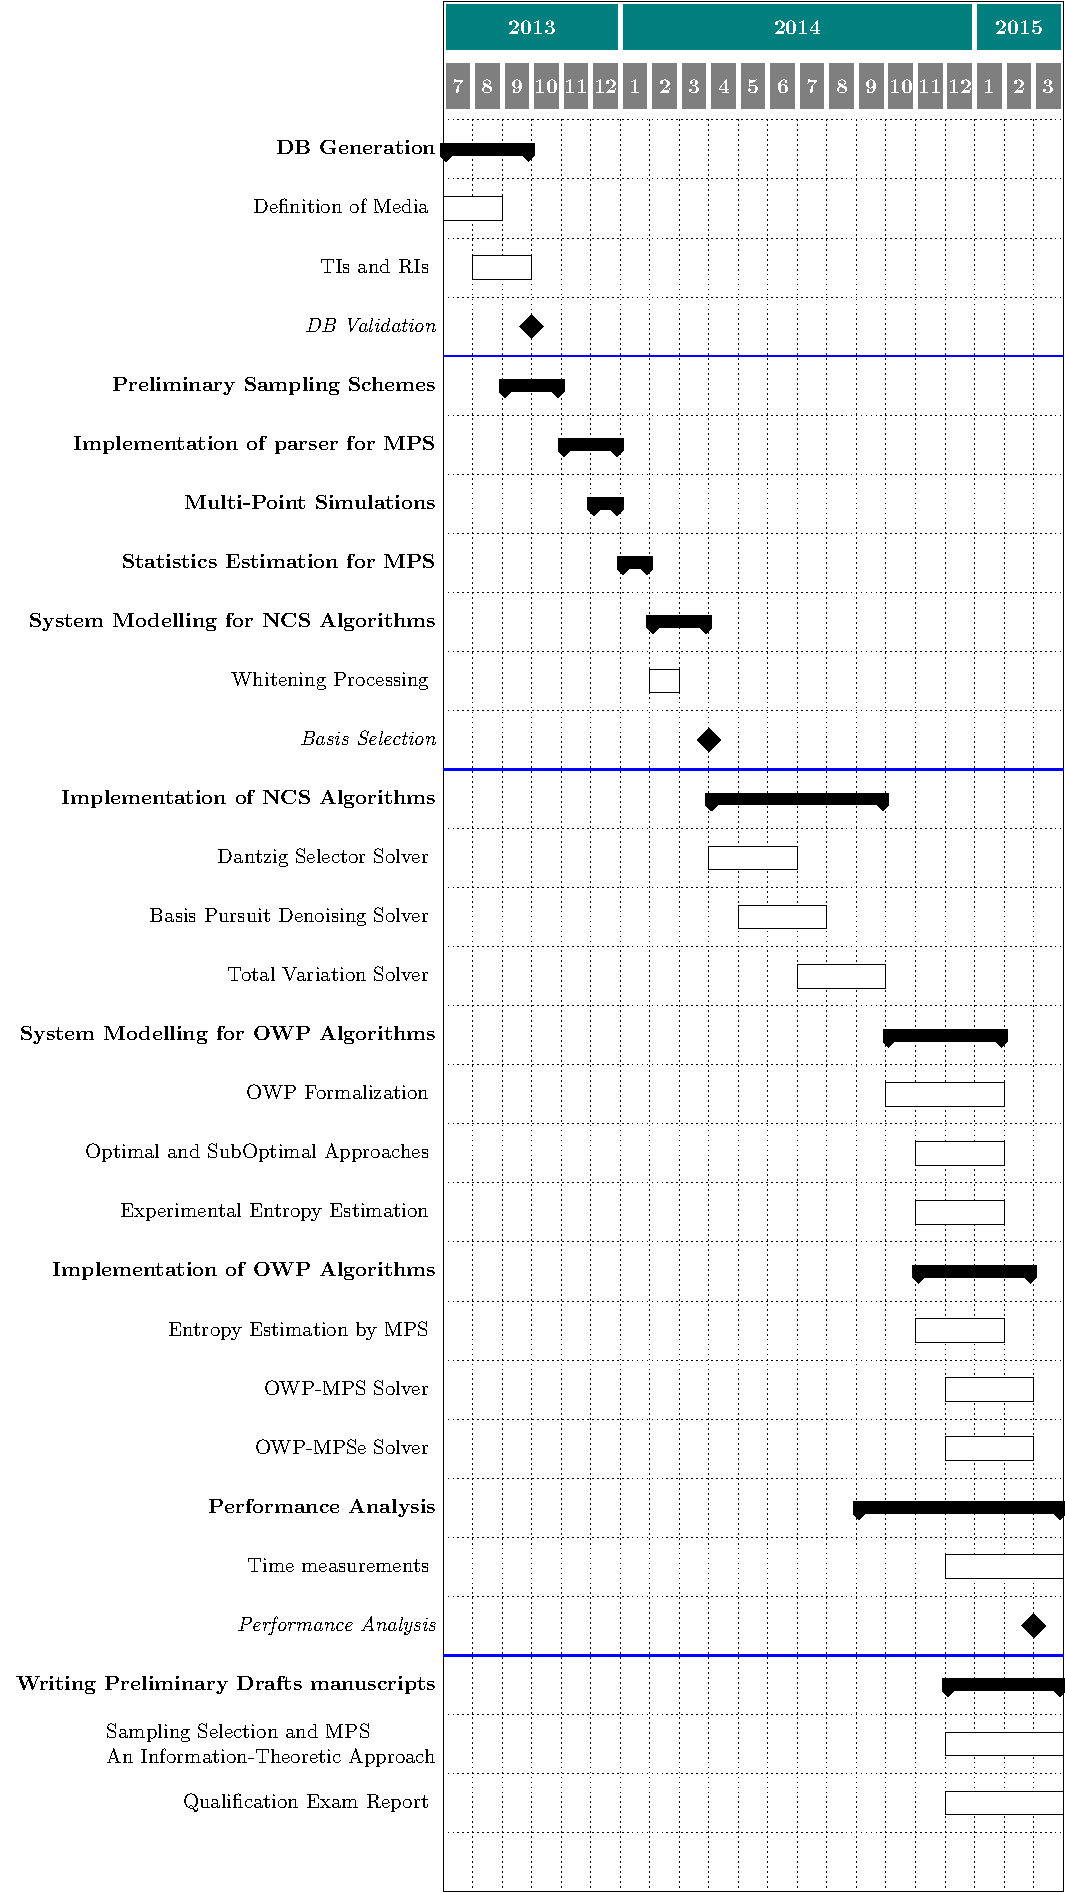
\includegraphics[width=.78\columnwidth]{Figures/_04_RoadMap/RoadMap1.pdf}
	\caption{\label{fig:RoadMap1} Gannt Chart for Preliminary Work}
 \end{figure}



\begin{figure}[ht!]
    \centering
    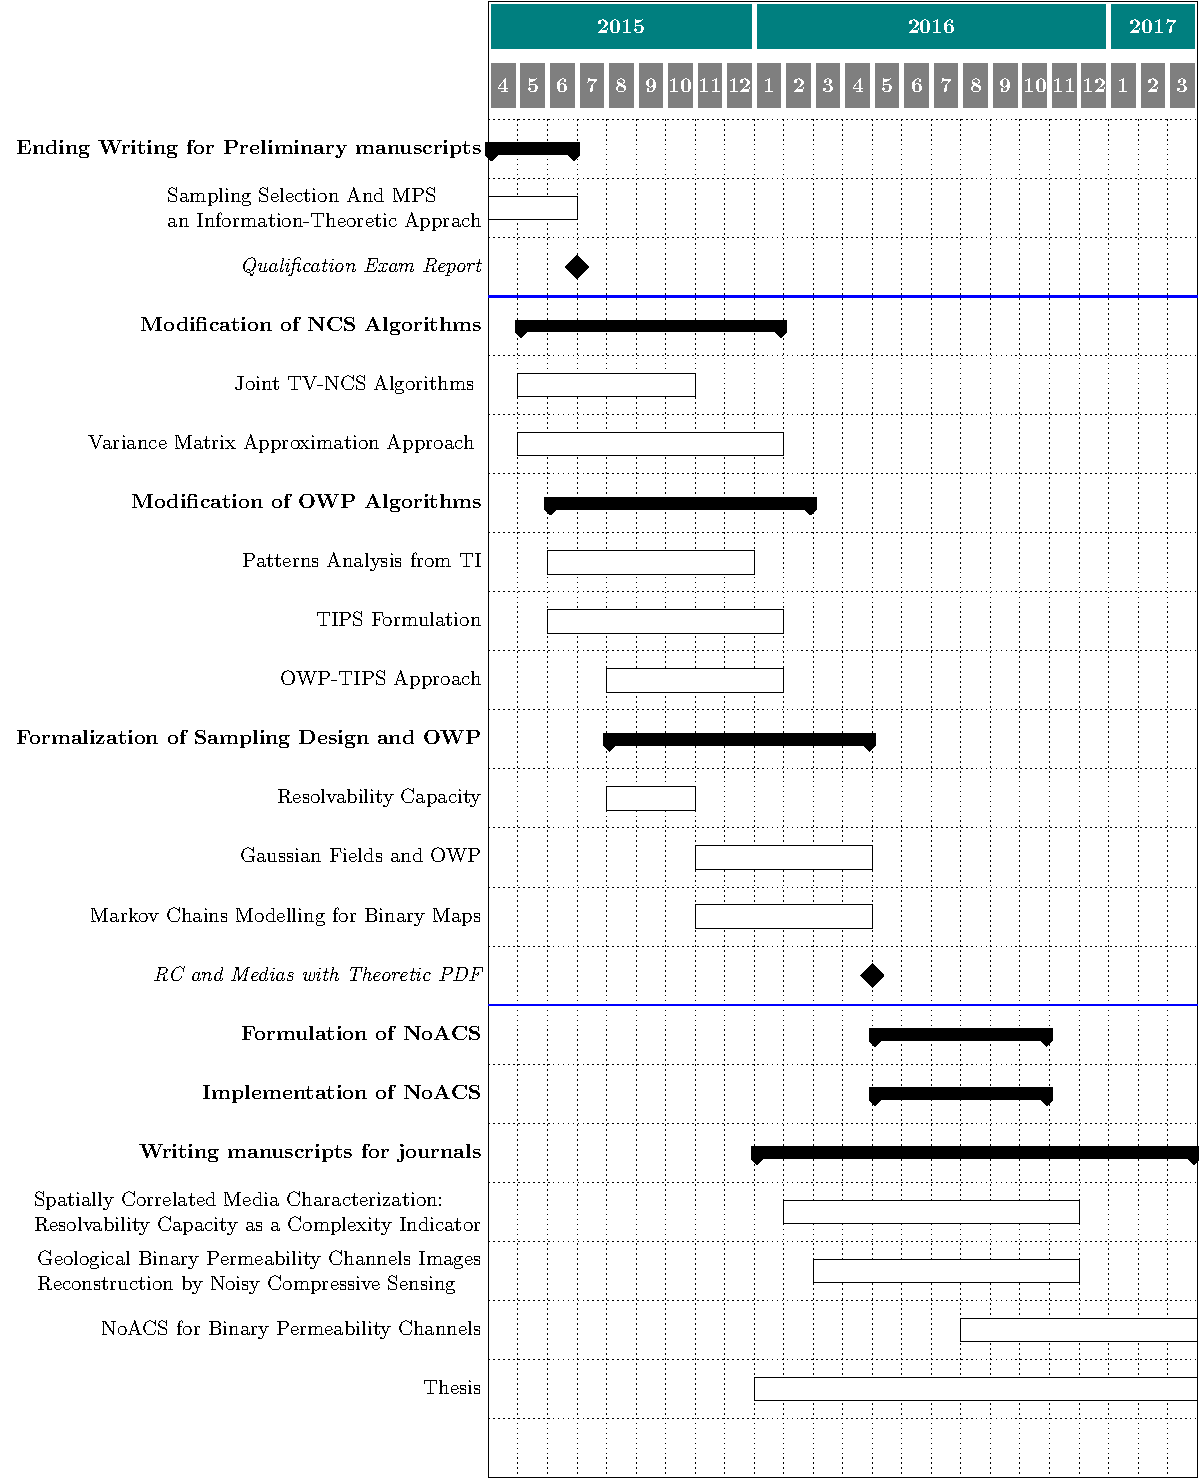
\includegraphics[width=1.0\columnwidth]{Figures/_04_RoadMap/RoadMap2.pdf}
	\caption{\label{fig:RoadMap2} Gannt Chart for Current and Future Work}
 \end{figure}

